%
% overall.tex
%
% Copyright (C) 2020 by SpaceLab.
%
% GOLDS-UFSC Documentation
%
% This work is licensed under the Creative Commons Attribution-ShareAlike 4.0
% International License. To view a copy of this license,
% visit http://creativecommons.org/licenses/by-sa/4.0/.
%

%
% \brief Overall description chapter.
%
% \author Gabriel Mariano Marcelino <gabriel.mm8@gmail.com>
%
% \institution Universidade Federal de Santa Catarina (UFSC)
%
% \version 0.1.0
%
% \date 2020/06/05
%

\chapter{Overall Description} \label{ch:overall}

.

\section{General Diagrams}

.

\section{General Behaviour}

.

\section{Orbit Parameters}

.

\section{Power Budget}

.

\section{Link Budget}

\subsection{VHF Link}

\begin{itemize}
    \item Direction: \textbf{Downlink}
    \item Frequency: \textbf{145,97 MHz}
    \item Modulation: \textbf{MSK}
    \item Datarate: \textbf{1200 bps}
    \item Output Power: \textbf{30 dBm (1 W)}
    \item Protocol: \textbf{NGHam}
\end{itemize}

\subsection{UHF Links}

\subsubsection{Main UHF Link}

\begin{itemize}
    \item Direction: \textbf{Downlink and uplink}
    \item Frequency: \textbf{436,9 MHz}
    \item Modulation: \textbf{MSK}
    \item Datarate: \textbf{4800 bps}
    \item Output power: \textbf{30 dBm (1 W)}
    \item Protocol: \textbf{NGHam}
\end{itemize}

\subsubsection{EDC UHF Link}

\begin{itemize}
    \item Direction: \textbf{Uplink}
    \item Frequency: \textbf{401.635 MHz}
    \item Modulation: \textbf{????}
    \item Datarate: \textbf{???? bps}
\end{itemize}

\section{PC-104 Bus}

\begin{figure}[!ht]
    \begin{center}
        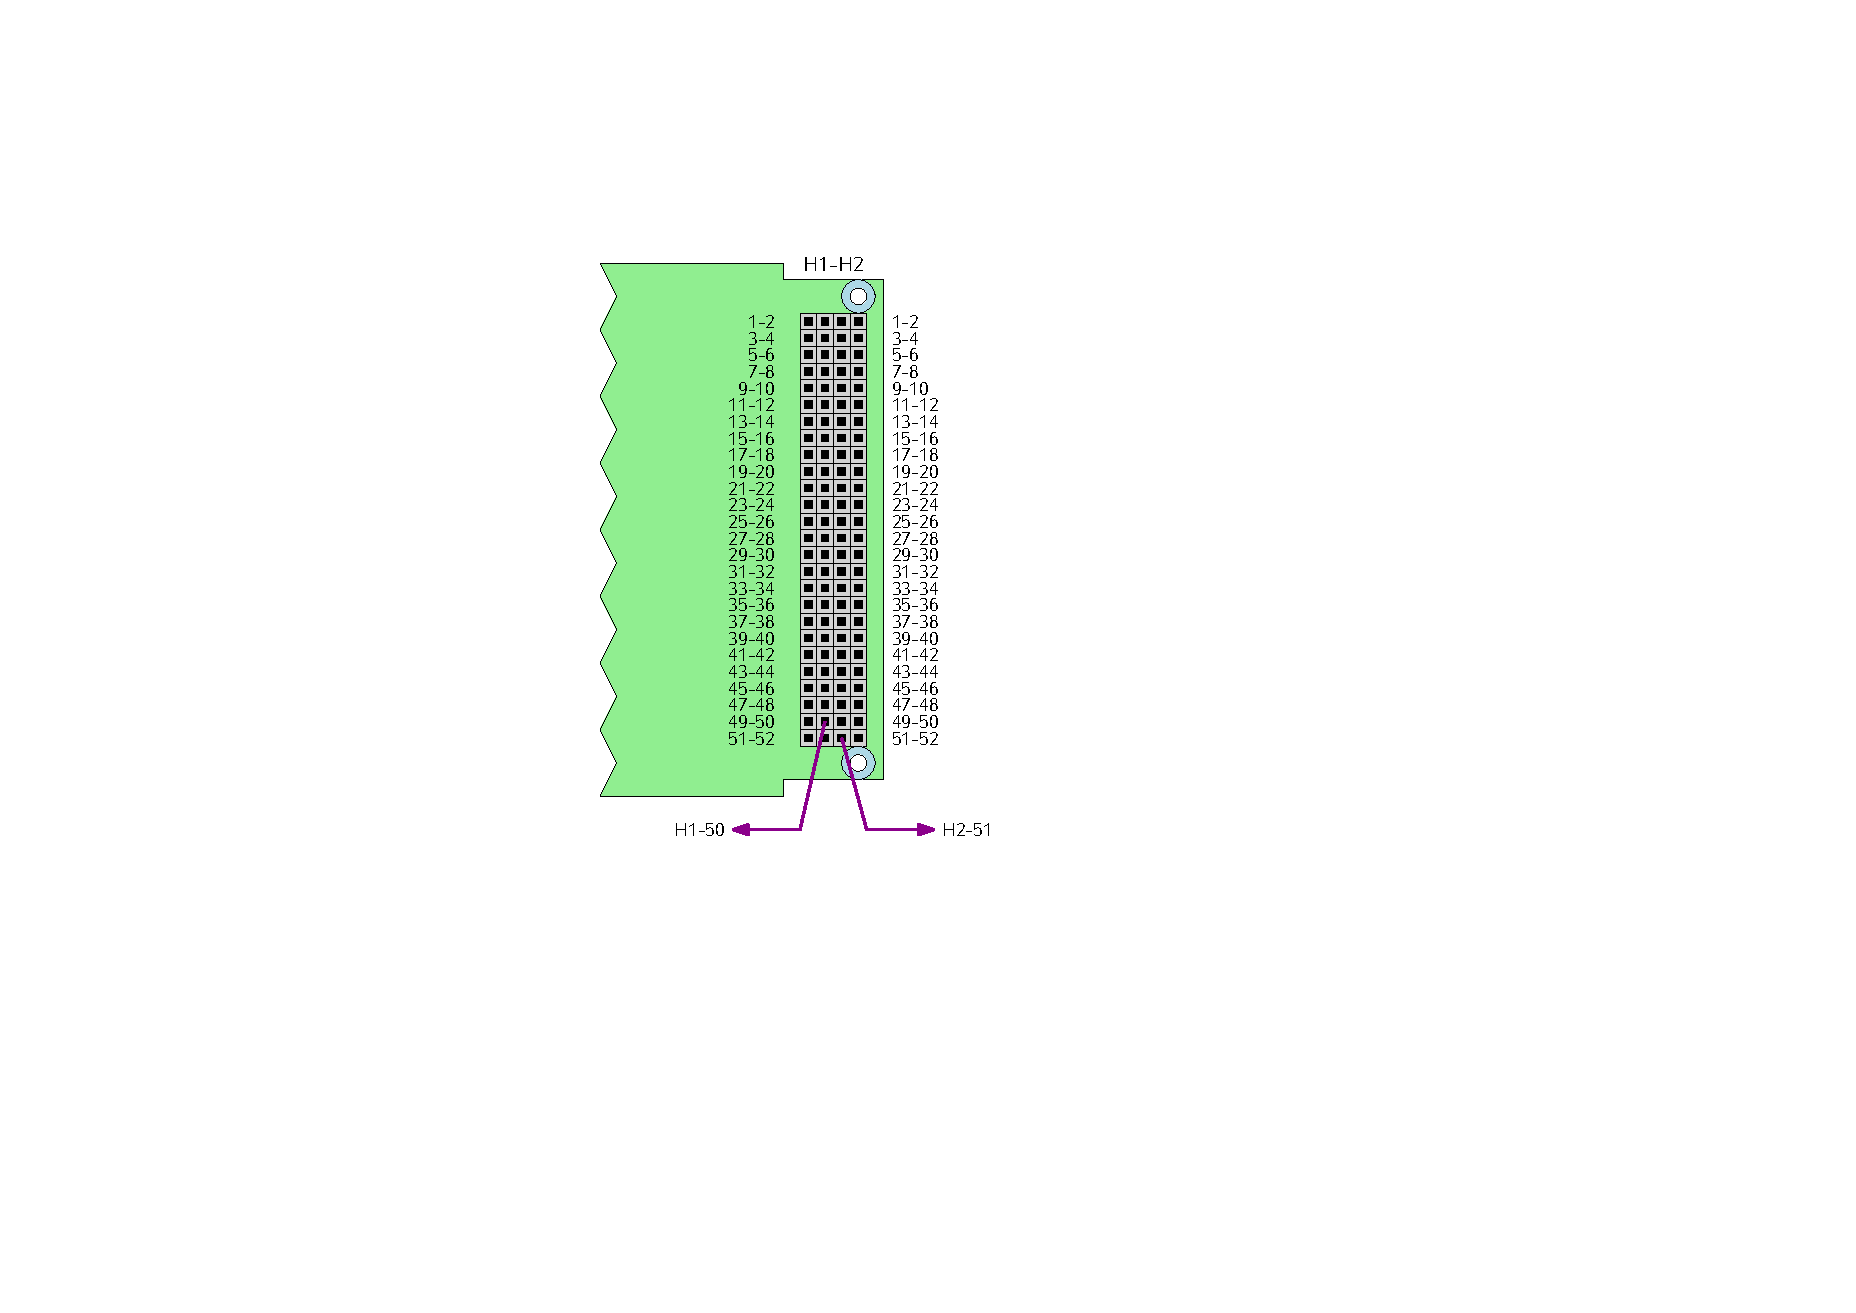
\includegraphics[width=0.5\textwidth]{figures/pc104-diagram}
        \label{fig:pc104-diagram}
        \caption{Reference diagram of the PC-104 bus.}
    \end{center}
\end{figure}

\begin{table}[!h]
    \centering
    \begin{tabular}{cllll}
        \toprule[1.5pt]
        \textbf{Pin Row}   & \textbf{H1 Odd}  & \textbf{H1 Even} & \textbf{H2 Odd} & \textbf{H2 Even} \\
        \midrule
        1-2                & -                & -                & -               & -                \\
        3-4                & -                & -                & -               & -                \\
        5-6                & -                & -                & BE\_UART\_RX    & -                \\
        7-8                & -                & -                & BE\_UART\_TX    & -                \\
        9-10               & -                & -                & -               & -                \\
        11-12              & -                & -                & BE\_SPI\_MOSI   & BE\_SPI\_CLK     \\
        13-14              & -                & -                & BE\_SPI\_CS     & BE\_SPI\_MISO    \\
        15-16              & -                & -                & -               & -                \\
        17-18              & -                & PLX\_EN          & -               & -                \\
        19-20              & -                & -                & -               & -                \\
        21-22              & -                & -                & -               & -                \\
        23-24              & -                & -                & -               & -                \\
        25-26              & EDC\_UART\_TX    & -                & -               & -                \\
        27-28              & EDC\_UART\_RX    & -                & -               & -                \\
        29-30              & GND              & GND              & GND             & GND              \\
        31-32              & GND              & GND              & GND             & GND              \\
        33-34              & -                & -                & -               & -                \\
        35-36              & RD\_SPI\_CLK     & -                & ANT\_VCC        & ANT\_VCC         \\
        37-38              & RD\_SPI\_MISO    & -                & -               & -                \\
        39-40              & RD\_SPI\_MOSI    & RD\_SPI\_CS      & -               & -                \\
        41-42              & PLX\_I2C\_SDA    & -                & -               & -                \\
        43-44              & PLX\_I2C\_SCL    & -                & -               & -                \\
        45-46              & OBDH\_VCC        & OBDH\_VCC        & BAT\_VCC        & BAT\_VCC         \\
        47-48              & EDC\_VCC         & EDC\_VCC         & -               & -                \\
        49-50              & RD\_VCC          & RD\_VCC          & EPS\_I2C\_SDA   & -                \\
        51-52              & BE\_VCC          & BE\_VCC          & EPS\_I2C\_SCL   & -                \\
        \bottomrule[1.5pt]
    \end{tabular}
    \caption{PC-104 bus pinout.}
    \label{tab:pc104-pinout}
\end{table}

\begin{table}[!h]
    \centering
    \begin{tabular}{lL{0.2\textwidth}L{0.15\textwidth}L{0.35\textwidth}}
        \toprule[1.5pt]
        \textbf{Signal} & \textbf{Pin(s)} & \textbf{Used By}     & \textbf{Description} \\
        \midrule
        GND             & H1-29, H1-30, H1-31, H1-32, H2-29, H2-30, H2-31, H2-32 & All                  & Ground reference \\
        BAT\_VCC        & H2-45, H2-46    & EPS                  & Battery terminals (+) \\
        ANT\_VCC        & H2-35, H2-36    & EPS, ANT             & Antenna power supply (3.3 V) \\
        OBDH\_VCC       & H1-45, H1-46    & EPS, OBDH            & OBDH power supply (3.3 V) \\
        EDC\_VCC        & H1-47, H1-48    & EPS, EDC             & EDC power supply (5 V) \\
        RD\_VCC         & H1-49, H1-50    & EPS, TTC             & Main radio power supply (5 V) \\
        BE\_VCC         & H1-51, H1-52    & EPS, TTC             & Beacon power supply (5 V) \\
        RD\_SPI\_CLK    & H1-35           & OBDH, TTC            & CLK signal of the main radio SPI bus \\
        RD\_SPI\_MISO   & H1-37           & OBDH, TTC            & MISO signal of the main radio SPI bus \\
        RD\_SPI\_MOSI   & H1-39           & OBDH, TTC            & MOS signal of the main radio SPI bus \\
        RD\_SPI\_CS     & H1-40           & OBDH, TTC            & CS signal of the main radio SPI bus \\
        EPS\_I2C\_SDA   & H2-49           & OBDH, EPS            & SDA signal of the EPS I2C bus \\
        EPS\_I2C\_SCL   & H2-51           & OBDH, EPS            & SCL signal of the EPS I2C bus \\
        BE\_UART\_RX    & H2-5            & EPS, TTC             & EPS TX, Beacon RX (UART bus) \\
        BE\_UART\_TX    & H2-7            & EPS, TTC             & EPS RX, Beacon TX (UART bus) \\
        EDC\_UART\_TX   & H1-25           & OBDH, EDC            & OBDH RX, EDC TX (UART bus) \\
        EDC\_UART\_RX   & H1-27           & OBDH, EDC            & OBDH TX, EDC RX (UART bus) \\
        PLX\_EN         & H1-18           & OBDH, Payload X      & Payload X enable (GPIO) \\
        PLX\_I2C\_SDA   & H1-41           & OBDH, Payload X      & SDA signal of the Payload X I2C bus \\
        PLX\_I2C\_SCL   & H1-43           & OBDH, Payload X      & SCL signal of the Payload X I2C bus \\
        \bottomrule[1.5pt]
    \end{tabular}
    \caption{PC-104 bus signal description.}
    \label{tab:pc104-signals}
\end{table}
